So now we get to roughly deriving the Einstein field equations. A few notes: this is not at all rigorous. At points, you may wonder why we are doing
something, but it will come back to the equations. I will try to provide as much intuition as possible, but you will need to understand
at least a decent amount of what we have done so far. So, here goes.
\subsection{Metric Tensor}
Let's start by imagining a grassy field, something like the one shown below.
\begin{figure}[H]
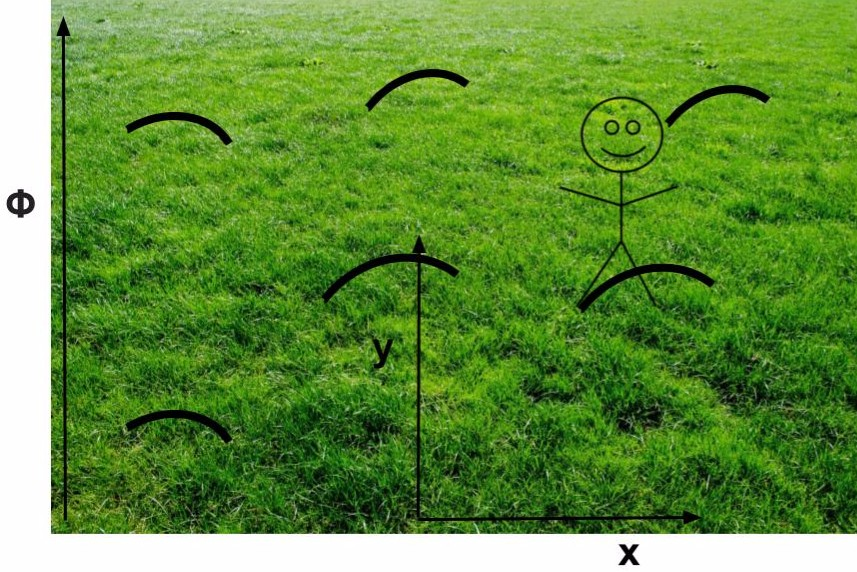
\includegraphics[scale=0.25]{field.jpg}
\end{figure}
Our grassy field is very bumpy, and so we want to find the height of the field (above sea level) where the person is standing. Well, to do so, first we must describe where the person is standing, so we impose a coordinate system, with an x and y axis, to show where our person is standing.
We also use $\phi$ to represent the height of the field at any one point. 
Now, suppose I ask you, if I moved, how much my height would change. Hopefully you would respond that it depends on the direction
of my movement. This point we will need for later: the direction of movement matters when considering this question.

Let's forget about the field for a moment and think about something called a gradient.
\begin{figure}[H]
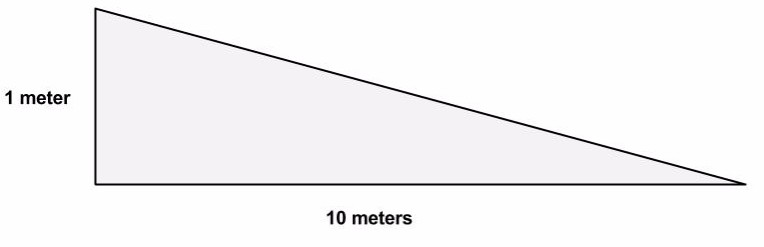
\includegraphics[scale=0.25]{gradient.jpg}
\end{figure}
A gradient is kind of like the scale on a map - it relates one distance to another. In our case, though, it relates the distance we walk to the change in height. In the gradient shown above, if we move 10 meters forward, we lose a meter in height. We can describe this gradient more generally using calculus. 
\begin{equation*}
d\phi=\frac{d\phi}{dx}dx
\end{equation*}
What does this equation mean? Well, on the left hand side, the term $d\phi$ means change in $\phi$, or, in our case, change in height. So, the change in height is equal to what? Well, the first term on the right hand side of the equation is change in height with respect to change in $x$, or our position. Really, this term represents the gradient! The next term merely means change in position, so we are saying that change in height is equal to the gradent multiplied by the change in position.
Let's test this with our gradient. Let's say we move $5$ meters. $d\phi=\frac{1}{10}\cdot 5$, which equals $\frac{1}{2}$. This makes sense, right? Just looking at the gradient intuitively we can see this.
Now, returning to our field, because the field is so bumpy, there is no clear gradient, but over very small distances this gradient could be true. So that is why we are using calculus (to some extent) here, we are dealing with very small quantities.
You'll also remember that we said earlier that direction matters. So instead of looking at change in height overall, let's say we look at change in height when we move in the $x$ direction and change in height when we move in the $y$ direction.
\begin{equation*}
d\phi_x=\frac{d\phi}{dx}dx
\end{equation*}
The above equation describes how height changes in the $x$ direction. Notice where $x$ shows up in the equation. We can replace these occurences with $y$ and get
\begin{equation*}
d\phi_y=\frac{d\phi}{dy}dy
\end{equation*}
Now, let's imagine that the person on the field is tired of moving in just the $x$ or $y$ direction. They want to go in a new direction, like shown below.
\begin{figure}[H]
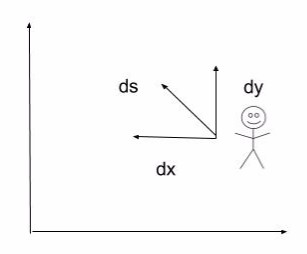
\includegraphics[scale=0.5]{sdir.jpg}
\end{figure}
How can we describe the change in height over that direction, $s$? Well, if you'll remember from the linear algebra section, we can treat vectors as combinations of other vectors. So what if we did that with this direction, composing it of the $x$ and $y$ directions?
This would give us the equation $d\phi_s=d\phi_x+d\phi_y$, which, if you plug in the numbers given in the earlier equations, gives
\begin{equation*}
d\phi_s=\frac{\partial\phi}{\partial x}\partial x+\frac{\partial\phi}{\partial y}\partial y
\end{equation*}
Notice how we switch to the partial derivative symbol, because we're dealing with multiple variables.

Now we're going to do a quick coordinate change, from $x$ and $y$ to $x^1$ and $x^2$ respectively. Why? Well, it is simpler to add extra dimensions this way. If we were to add extra letters, it is more difficult, because letters often have specific meanings in physics and so could be construed for something else. However, there are an infinite number of numbers, so we can simply, if adding a third dimension, call it $x^n$. So, substituting in these coordinates, we get
\begin{equation*}
    d\phi= \frac{\partial \phi}{\partial x^1}\partial x^1+\frac{\partial\phi}{\partial x^2}dx^2+...
\end{equation*}
The reason for the $+...$ is merely to account for other dimensions. Now, we can rewrite this equation using summation notation, getting
\begin{equation}
    d\phi=\sum\limits_n\frac{\partial\phi}{\partial x^n}dx^n
\end{equation}
(We'll be referencing this equation later as equation one.) Note that all the sum notation is is a way to represent the fact that we are adding all of the different dimensions (all of the components of whichever direction we are going).

Now, let's consider a different situation: what if we have a different coordinate system, $y^1$ and $y^2$, and we wish to convert between $\frac{\partial\phi}{\partial x^n}$ and $\frac{\partial\phi}{\partial y^n}$. How could we do that? (Let's imagine that the $y$ coordinate system looks something like that in the diagram shown below.)
\begin{figure}[H]
    \centering
    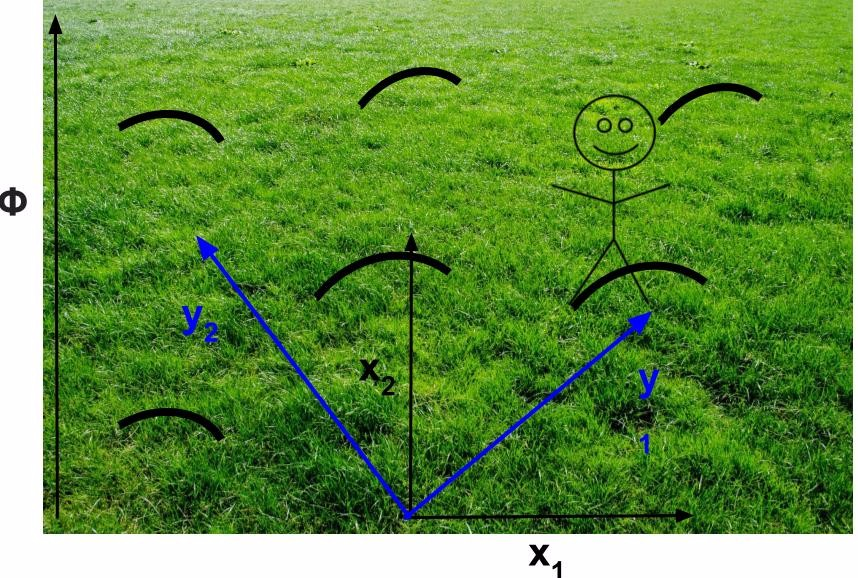
\includegraphics{newcor.jpg}
\end{figure}
Note that to identify a $y^1$ coordinate in the $x$ system, one needs two $x$ coordinates. One can convert using the equation 
\begin{equation*}
    \frac{\partial\phi}{\partial y^1}=\frac{\partial\phi}{x^1}\frac{\partial x^1}{\partial y^1}+\frac{\partial\phi}{\partial x^2}\frac{\partial x^2}{y^1}
\end{equation*}
which can be further reduced to
\begin{equation}
    \frac{\partial\phi}{\partial y^n}=\sum\limits_m\frac{\partial\phi}{\partial x^m}\frac{\partial x^m}{\partial y^n}
\end{equation}
We'll refer to this equation later as equation two. Now, we must enter a brief interlude to continue.
\section{Tensors}
We have already talked about, in the chapter on linear algebra, scalars and vectors. Tensors are a further generalization of vectors. Scalars are tensors of rank 0, vectors are tensors of rank 1, matrices are tensors of rank 2, and so on. There are multiple ways one can define a tensor, but here, we'll define a tensor as a function that takes in vectors and spits out a scalar. (Another way of describing a tensor is that it takes only one number to pick out an individual component of a vector, hence, vectors are rank one tensors. In other words, the number of indices needed to pick out a component of a tensor defines that tensor's rank.)

Now, keeping this in mind, let us rewrite equation one replacing $d\phi$ and $dx$ with vectors. This gives the equation
\begin{equation}
    V^n_y=\sum\limits_m\frac{dy^n}{dx^m}V^m_x
\end{equation}
(We'll refer to this equation as equation three.) 
Let's consider a combination of vectors. Let's take vector $A$, and the $n$th coordinate of that vector $A^n$, and then take another vector $B$ and then take the $m$th coordinate, $B^m$. If we multiply these two together, we get a tensor, $T^{mn}$. Further, if we use equation three, we can create the new equation 
\begin{equation*}
    A_y^mB_y^n=\sum\limits_r\frac{\partial y^m}{\partial x^r}A_x^r \sum\limits_s\frac{\partial y^n}{\partial x^s} B_x^s
\end{equation*}
which can then be rewritten as 
\begin{equation}
    T_y^{mn}=\sum\limits_{rs}\frac{\partial y^m}{\partial x^r}
\end{equation}
